% Created 2021-07-16 Fri 03:37
% Intended LaTeX compiler: pdflatex
\documentclass[11pt]{article}
\usepackage[utf8]{inputenc}
\usepackage[T1]{fontenc}
\usepackage{graphicx}
\usepackage{grffile}
\usepackage{longtable}
\usepackage{wrapfig}
\usepackage{rotating}
\usepackage[normalem]{ulem}
\usepackage{amsmath}
\usepackage{textcomp}
\usepackage{amssymb}
\usepackage{capt-of}
\usepackage{hyperref}
\linespread{1.5}
\usepackage[margin=1.5in]{geometry}
\usepackage{mathptmx}
\date{\today}
\title{}
\hypersetup{
 pdfauthor={},
 pdftitle={},
 pdfkeywords={},
 pdfsubject={},
 pdfcreator={Emacs 27.2 (Org mode 9.4.4)}, 
 pdflang={English}}
\begin{document}

\tableofcontents

\clearpage
\section{Introduction}
\label{sec:org1f0210d}
\subsection{What is Natural Language Processing}
\label{sec:orgc727206}
\textbf{Natural language processing} (NLP) refers to the branch of \textbf{computer science} and more
specifically, the branch of \textbf{artificial intelligence} or AI concerned with giving computers
the ability to understand text and spoken words in much the same way human beings can.

\begin{figure}[htbp]
\centering
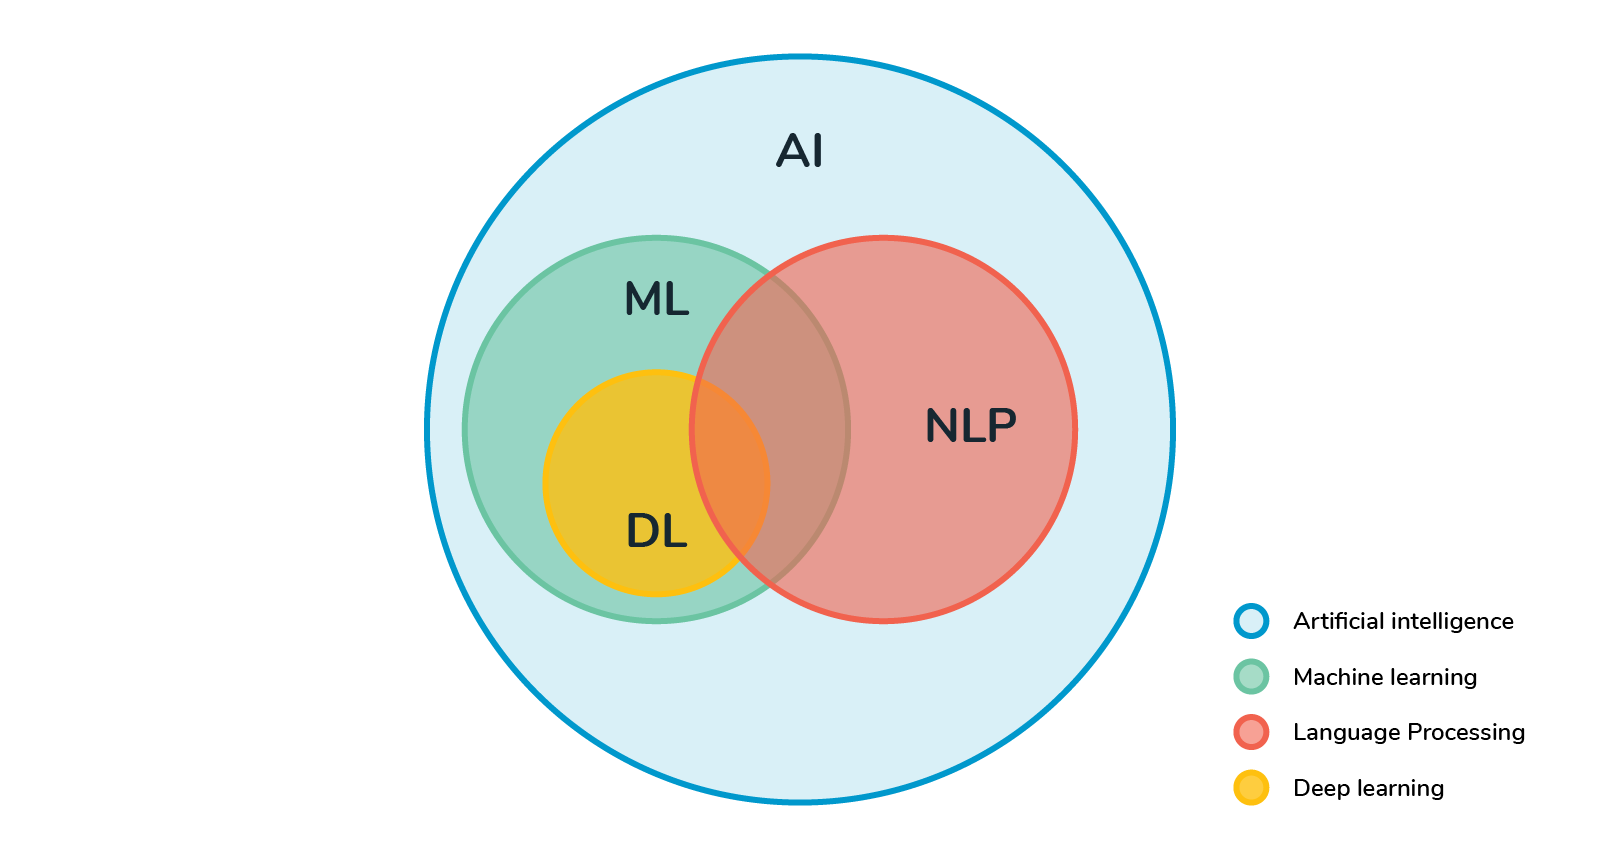
\includegraphics[width=.9\linewidth]{./img/nlp.png}
\caption{\label{fig:org26225df}NLP is subfield of AI}
\end{figure}

NLP combines \emph{computational linguistics} rule-based modeling of human language with
statistical, machine learning, and deep learning models. Together, these technologies
enable computers to process human language in the form of text or voice data and to
‘understand’ its full meaning, complete with the speaker or writer’s intent and sentiment.

\subsection{Why NLP is so Important}
\label{sec:org12e8316}
In a world of Google and other search engines, shoppers expect to enter a phrase,
or even an idea, into a search box and to instantly see personalized recommendations
that are clearly relevant to what it was they were meaning to discover.
It’s the sort of interaction that must go on at a speed and scale that can’t be
sustained by humans alone.
\begin{figure}[htbp]
\centering
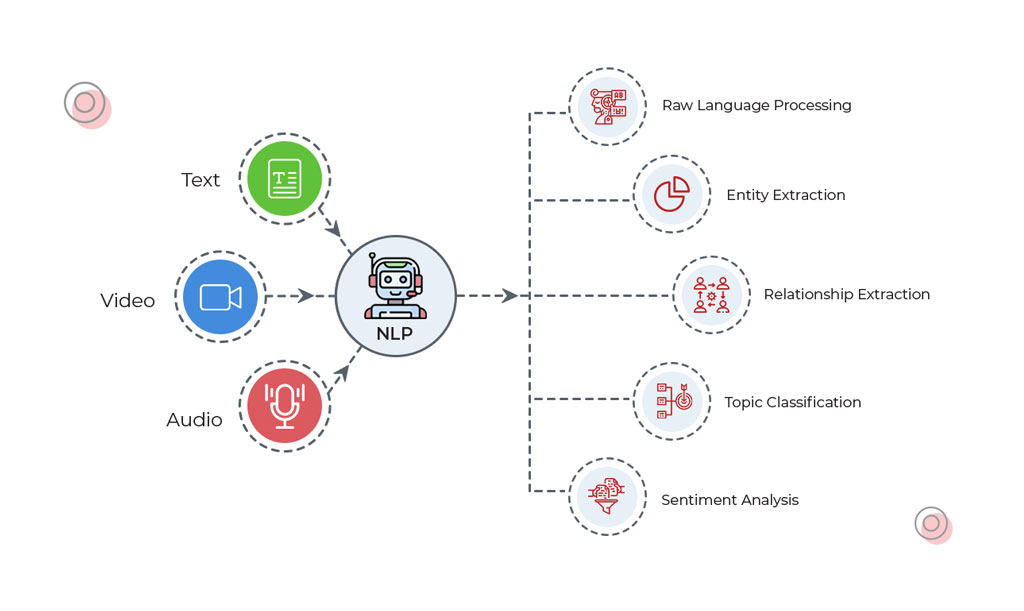
\includegraphics[width=.9\linewidth]{./img/nlp-paper.png}
\caption{\label{fig:org1ee1670}NLP functioning}
\end{figure}
Instead, doing right by consumers requires machines and systems that are constantly
learning and developing insights into what customers mean and what they want.

\subsection{Computational linguistics}
\label{sec:org6e834cd}
It is the modern study of linguistics using the tools of computer science. Yesterday’s
linguistics may be today’s computational linguist as the use of computational tools
and thinking has overtaken most fields of study.
\clearpage

\section{NLP Tasks}
\label{sec:orgf014584}
Human language is filled with ambiguities that make it incredibly difficult to write
software that accurately determines the intended meaning of text or voice data.
Homonyms, homophones, sarcasm, idioms, metaphors, grammar and usage exceptions,
variations in sentence structure—these just a few of the irregularities of human
language that take humans years to learn, but that programmers must teach natural
language-driven applications to recognize and understand accurately from the start,
if those applications are going to be useful.

Several NLP tasks break down human text and voice data in ways that help the computer
make sense of what it's ingesting. Some of these tasks include the following:

\subsection{Speech recognition (aka speech-to-text)}
\label{sec:orgaab8843}
It is the task of reliably converting voice data into text data.
Speech recognition is required for any application that follows voice commands or
answers spoken questions. What makes speech recognition especially challenging is
the way people talk—quickly, slurring words together, with varying emphasis and
intonation, in different accents, and often using incorrect grammar.

\subsection{Part of speech tagging}
\label{sec:org4833f63}
It is the process of determining the part of speech of a particular word or
piece of text based on its use and context. Part of speech identifies ‘make’ as a
verb in ‘I can make a paper plane,’ and as a noun in ‘What make of car do you own?’

\subsection{Word sense disambiguation}
\label{sec:orgde4fb7c}
It is the selection of the meaning of a word with multiple meanings through a process
of semantic analysis that determine the word that makes the most sense in the given
context. For example, word sense disambiguation helps distinguish the meaning of the
verb 'make' in ‘make the grade’ (achieve) vs. ‘make a bet’ (place).

\subsection{Sentiment analysis}
\label{sec:org55be584}
Some attempts to extract subjective qualities—attitudes, emotions, sarcasm, confusion,
suspicion—from text. Basically understanding human emotions.
\begin{figure}[htbp]
\centering
\includegraphics[width=.9\linewidth]{./img/sentiment.png}
\caption{\label{fig:org79524c0}Sentiment detection}
\end{figure}   

\subsection{Natural language generation}
\label{sec:org8815008}
It is sometimes described as the opposite of speech recognition or speech-to-text;
it's the task of putting structured information into human language. 

\clearpage

\section{NLP Challenges}
\label{sec:org00bcdc1}
NLP is a powerful tool with huge benefits, but there are still a number of Natural
Language Processing limitations and problems:
\subsection{Contextual words and phrases and homonyms}
\label{sec:orgfc7c0cd}
The same words and phrases can have different meanings according the context of a sentence and many words – especially in English – have the exact same pronunciation but totally different meanings.
For example:
I ran to the store because we ran out of milk.
Can I run something past you real quick?
The house is looking really run down.
These are easy for humans to understand because we read the context of the sentence and we understand all of the different definitions. And, while NLP language models may have learned all of the definitions, differentiating between them in context can present problems.
Homonyms – two or more words that are pronounced the same but have different definitions – can be problematic for question answering and speech-to-text applications because they aren’t written in text form. Usage of their and there, for example, is even a common problem for humans.  

\subsection{Synonyms}
\label{sec:orgdd202d8}
Synonyms can lead to issues similar to contextual understanding because we use
many different words to express the same idea. Furthermore, some of these words
may convey exactly the same meaning, while some may be levels of complexity
(small, little, tiny, minute) and different people use synonyms to denote slightly
different meanings within their personal vocabulary.
\subsection{Irony and sarcasm}
\label{sec:org21593f6}
Irony and sarcasm present problems for machine learning models because they generally
use words and phrases that, strictly by definition, may be positive or negative, but
actually connote the opposite.
Models can be trained with certain cues that frequently accompany ironic or sarcastic
phrases, like \emph{“yeah right,” “whatever,”} etc., and word embeddings (where words that
have the same meaning have a similar representation), but it’s still a tricky process.
\subsection{Ambiguity}
\label{sec:orge416433}
Even for humans this sentence alone is difficult to interpret without
the context of surrounding text. POS (part of speech) tagging is one NLP solution
that can help solve the problem, somewhat.
Ambiguity in NLP refers to sentences and phrases that potentially have two or more
possible interpretations.

\subsubsection{Lexical ambiguity}
\label{sec:orge93ba59}
A word that could be used as a verb, noun, or adjective.
\subsubsection{Semantic ambiguity}
\label{sec:org5c41a6a}
The interpretation of a sentence in context. For example: I saw the boy on the
beach with my binoculars. This could mean that I
\subsubsection{Syntactic ambiguity}
\label{sec:org0a57ef2}
In the sentence above, this is what creates the confusion of meaning.
The phrase with my binoculars could modify the verb, “saw,” or the noun, “boy.”

\subsection{Errors in text and speech}
\label{sec:org34b1e3a}
Misspelled or misused words can create problems for text analysis. Autocorrect and
grammar correction applications can handle common mistakes, but don’t always
understand the writer’s intention.
With spoken language, mispronunciations, different accents, stutters, etc., can
be difficult for a machine to understand. However, as language databases grow and
smart assistants are trained by their individual users, these issues can be minimized.
\subsection{Colloquialisms and slang}
\label{sec:orgdeb5f70}
Informal phrases, expressions, idioms, and culture-specific lingo present a number
of problems for NLP – especially for models intended for broad use. Because as formal
language, colloquialisms may have no “dictionary definition” at all, and these
expressions may even have different meanings in different geographic areas.
Furthermore, cultural slang is constantly morphing and expanding, so new words
pop up every day.
This is where training and regularly updating custom models can be helpful,
although it oftentimes requires quite a lot of data.
\subsection{Domain-specific language}
\label{sec:orgb64a009}
Different businesses and industries often use very different language. An NLP
processing model needed for healthcare, for example, would be very different than
one used to process legal documents. These days, however, there are a number of
analysis tools trained for specific fields, but extremely niche industries may need
to build or train their own models.
\subsection{Low-resource languages}
\label{sec:org82a93a2}
AI machine learning NLP applications have been largely built for the most common,
widely used languages. And it’s downright amazing at how accurate translation systems
have become. However, many languages, especially those spoken by people with less
access to technology often go overlooked and under processed. For example, by some
estimations, (depending on language vs. dialect) there are over 3,000 languages in
Africa, alone. There simply isn’t very much data on many of these languages.
\subsection{Lack of research and development}
\label{sec:org40cb9b7}
Machine learning requires A LOT of data to function to its outer limits – billions
of pieces of training data. The more data NLP models are trained on, the smarter
they become. That said, data (and human language!) is only growing by the day, as
are new machine learning techniques and custom algorithms. All of the problems above
will require more research and new techniques in order to improve on them.
Advanced practices like artificial neural networks and deep learning allow a multitude
of NLP techniques, algorithms, and models to work progressively, much like the human
mind does. As they grow and strengthen, we may have solutions to some of these
challenges in the near future.
\clearpage

\section{NLP use cases}
\label{sec:org31641a5}
Natural language processing is the driving force behind machine intelligence in
many modern real-world applications. Here are a few examples:
\subsection{Spam detection}
\label{sec:orgbf0b167}
You may not think of spam detection as an NLP solution, but the best spam detection
technologies use NLP's text classification capabilities to scan emails for language
that often indicates spam or phishing. These indicators can include overuse of
financial terms, characteristic bad grammar, threatening language, inappropriate
urgency, misspelled company names, and more. Spam detection is one of a handful
of NLP problems that experts consider 'mostly solved' (although you may argue that
this doesn’t match your email experience).

\subsection{Machine translation}
\label{sec:org8b6fce4}
Google Translate is an example of widely available NLP technology at work.
Truly useful machine translation involves more than replacing words in one language
with words of another.  Effective translation has to capture accurately the meaning
and tone of the input language and translate it to text with the same meaning and
desired impact in the output language. Machine translation tools are making good
progress in terms of accuracy. A great way to test any machine translation tool is
to translate text to one language and then back to the original.

\subsection{Social media sentiment analysis}
\label{sec:orga1c62ab}
NLP has become an essential business tool for uncovering hidden data insights from
social media channels. Sentiment analysis can analyze language used in social media
posts, responses, reviews, and more to extract attitudes and emotions in response
to products, promotions, and events–information companies can use in product designs,
advertising campaigns, and more.

\subsection{Text summarization}
\label{sec:org39f7cfc}
Text summarization uses NLP techniques to digest huge volumes of digital text and
create summaries and synopses for indexes, research databases, or busy readers who
don't have time to read full text. The best text summarization applications use
semantic reasoning and natural language generation (NLG) to add useful context
and conclusions to summaries.

\subsection{Virtual assistants and chatbots}
\label{sec:orgd5c9379}
Virtual assistants such as Apple's Siri and Amazon's Alexa use speech recognition
to recognize patterns in voice commands and natural language generation to respond
with appropriate action or helpful comments. Chatbots perform the same magic in
response to typed text entries. The best of these also learn to recognize contextual
clues about human requests and use them to provide even better responses or options
over time. 
\clearpage

\section{NLP tools and approaches}
\label{sec:org21d6c6e}
\begin{figure}[htbp]
\centering
\includegraphics[width=.9\linewidth]{./img/nlp-jumbo.png}
\caption{\label{fig:org5be45b6}NLP principles}
\end{figure}     
With the help of modern computer science tools and technology. NLP can be done easily.
Lot of high level library and framework are available publically to be used.

\subsection{Python and the Natural Language Toolkit (NLTK)}
\label{sec:org130ef89}
The Python programing language provides a wide range of tools and libraries
for attacking specific NLP tasks. Many of these are found in the Natural Language
Toolkit, or NLTK, an open source collection of libraries, programs, and
education resources for building NLP programs.
The NLTK includes libraries for many of the NLP tasks listed above, plus libraries
for subtasks, such as sentence parsing, word segmentation, stemming and
lemmatization (methods of trimming words down to their roots), and tokenization
(for breaking phrases, sentences, paragraphs and passages into tokens that help
the computer better understand the text). It also includes libraries for implementing
capabilities such as semantic reasoning, the ability to reach logical conclusions
based on facts extracted from text.

\subsection{Statistical NLP, machine learning, and deep learning}
\label{sec:orgd9f286d}
The earliest NLP applications were hand-coded, rules-based systems that could perform
certain NLP tasks, but couldn't easily scale to accommodate a seemingly endless stream
of exceptions or the increasing volumes of text and voice data.
Enter statistical NLP, which combines computer algorithms with machine learning and
deep learning models to automatically extract, classify, and label elements of text
and voice data and then assign a statistical likelihood to each possible meaning of
those elements. Today, deep learning models and learning techniques based on
convolutional neural networks (CNNs) and recurrent neural networks (RNNs) enable
NLP systems that 'learn' as they work and extract ever more accurate meaning from
huge volumes of raw, unstructured, and unlabeled text and voice data sets. 
\clearpage

\section{Products based on NLP}
\label{sec:org643b718}
\subsection{Amazon's Alexa}
\label{sec:org24a9c5f}
Alexa is Amazon’s all-knowing, interactive voice assistant. Available on Amazon’s
lineup of Echo speakers, smart thermostats, soundbars, lamps and lights, and right
on your phone through the Alexa app, Alexa can do quick math for you, launch your
favorite playlists, check news and weather, and control many of your home’s smart products.
In this guide, we explain where Alexa comes from, exactly how Alexa works, where
Alexa gets her name, and more.
\begin{figure}[htbp]
\centering
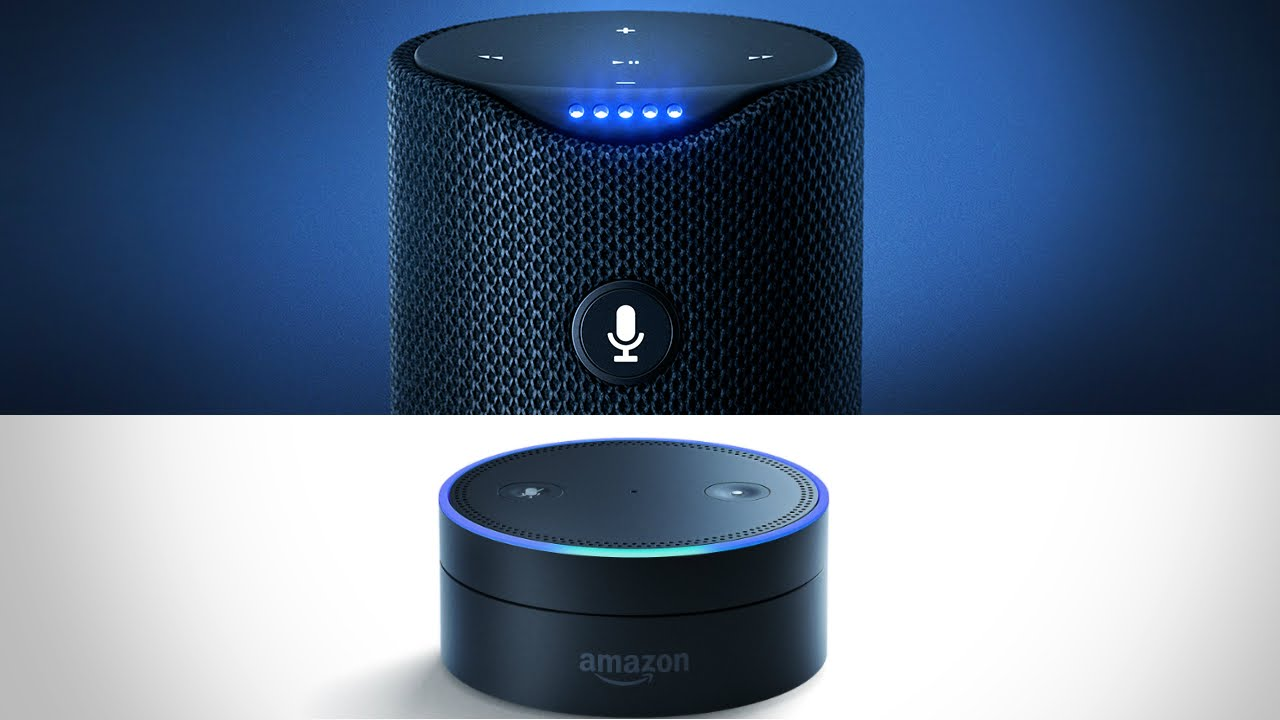
\includegraphics[width=.9\linewidth]{./img/alexa.png}
\caption{\label{fig:orgce10069}Variant alexa products by amazon}
\end{figure}   

\subsection{Apple's Siri}
\label{sec:org9fabae6}
Siri, Apple's personal digital assistant, uses machine learning and natural speech
to answer questions, return relevant search information, perform actions and more.
\begin{figure}[htbp]
\centering
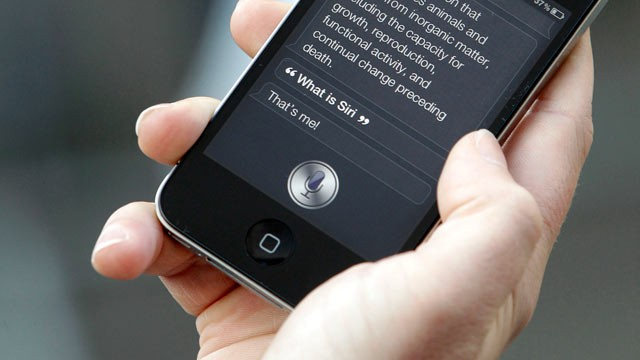
\includegraphics[width=.9\linewidth]{./img/siri.png}
\caption{\label{fig:orge7f73f8}Siri running on iPhone}
\end{figure}

\subsection{Google voice assistant}
\label{sec:orgb3de5cb}
Google Assistant offers voice commands, voice searching, and voice-activated
device control, letting you complete a number of tasks after you've said the
"OK Google" or "Hey Google" wake words. It is designed to give you conversational
interactions. Google Assistant will: Control your devices and your smart home
\begin{figure}[htbp]
\centering
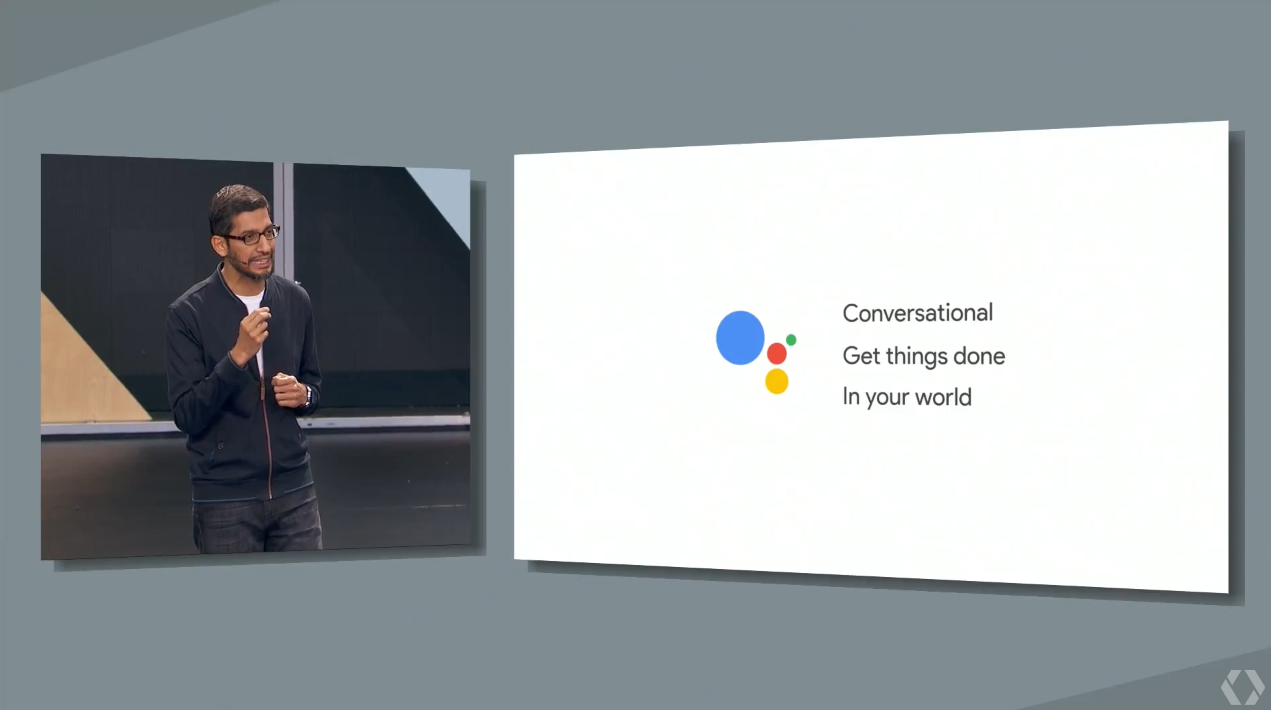
\includegraphics[width=.9\linewidth]{./img/google-assistant.png}
\caption{\label{fig:org51f6950}Sundar Pichai (CEO of google) introducing google assistant}
\end{figure}

\clearpage

\section{Lojban}
\label{sec:org7980681}
Lojban is a carefully constructed spoken language. It has been built for over 50
years by dozens of workers and hundreds of supporters.
\begin{figure}[htbp]
\centering
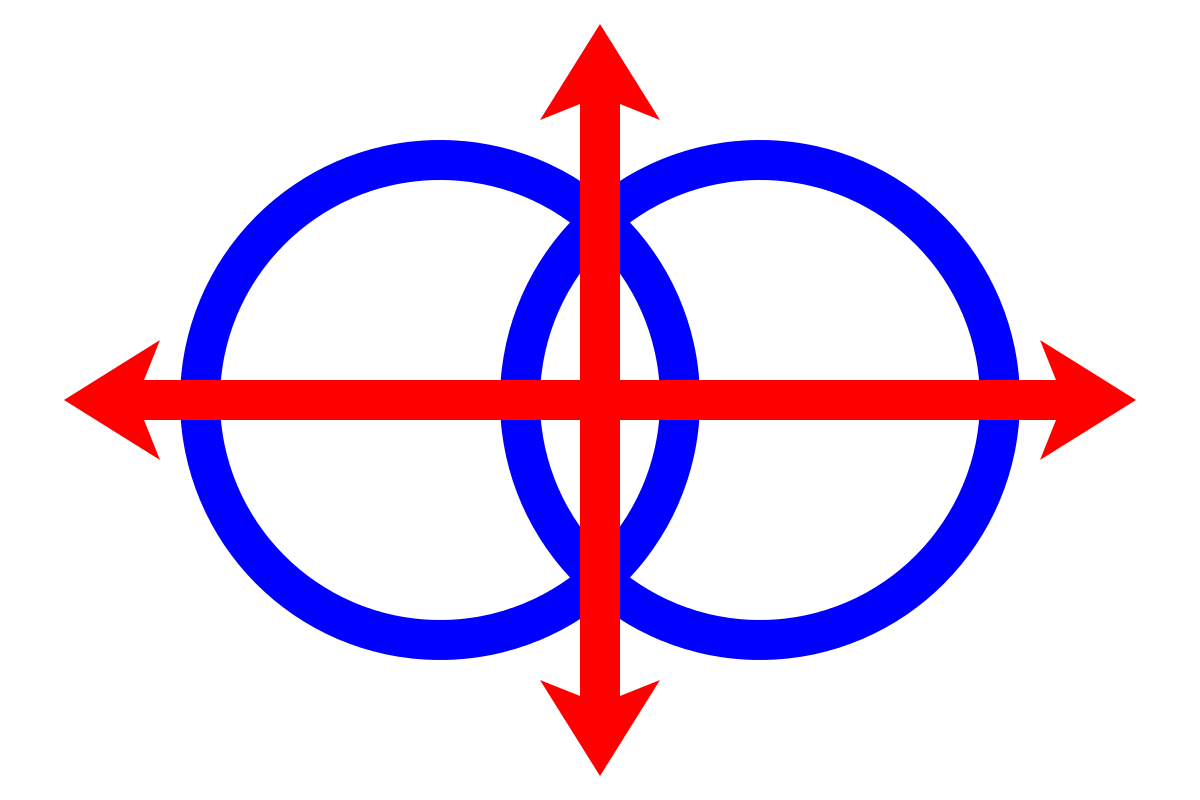
\includegraphics[width=.9\linewidth]{./img/lojban.png}
\caption{\label{fig:org2a8131a}Lojban logo}
\end{figure}
\begin{itemize}
\item Lojban's grammar is based on simple rules, and its linguistic features
are inspired by predicate logic.
\item Lojban allows the expression of nuances in emotion using words called attitudinals,
which are like spoken emoticons. ue marks that you're surprised; ba'u marks that
you're exaggerating.
\item You can be as vague or detailed as you like when speaking lojban.
For example, specifying tense (past, present or future) or number
(singular or plural) is optional when they're clear from context.
\item Lojban is machine parsable, so the syntactic structure and validity of a sentence
is unambiguous, and can be analyzed using computer tools.
\item There is a live community of speakers expanding the lojban vocabulary day by day.
\end{itemize}

\subsection{Lojban means different things to different people}
\label{sec:orga63b4d4}
\begin{itemize}
\item a linguistic curiosity - a test-bed for language experimentation
\item a challenging way to expand their minds or discipline their thoughts
\item a new perspective on languages
\item an entertaining medium to communicate with friends or create art
\item a domain for exploring the intersection of human language and software
\end{itemize}

\subsection{Lojban applications}
\label{sec:org08ed496}
While the initial aim of the Loglan project was to investigate linguistic relativity,
the active Lojban community recognizes additional applications for the language,
including:
\begin{itemize}
\item Improved human–human communication, due to the logical and unambiguous structure
and greater means of expression (use as a speakable language)
\begin{itemize}
\item Eliminating syntactic ambiguity in language
\end{itemize}
\item Use as an educational tool
\item Research in artificial intelligence and machine understanding
\begin{itemize}
\item Improved human–computer communication, storage ontologies, and computer
translation of natural language text
\end{itemize}
\item Research in linguistics
\item Use as an academic language, such as in science or philosophy
\end{itemize}
\clearpage

\section{Conclusion}
\label{sec:orgd89513c}
NLP and machine learning applications play a pivotal role in supporting machine-human
communications. With more research in this sphere, there are more developments to make
machines smarter at learning and understanding the human language.

NLP is one of the growing technologies. With constant innovation and research going
on in this field, it is only expected to grow in the future. Since this is such an
upcoming field, there is a dire need for skilled professionals. If you are interested
in working on making computers learn and understand human language, then this is a
good time to upskill yourself. NLP offers good prospects and is a high paying field.

Coding Elements offers courses in technologies like Python for Data Science, Data
Science with R, Machine Learning and Deep Learning, Full Stack Web Development, Mobile
App Development. Their curriculum is created based on the latest industry trends and
is taught by expert faculty. We provide the best LIVE classroom and Online classes.
The classes are very flexible and come with an access period of 4 years.
\clearpage

\section{References}
\label{sec:orgb7e235b}
\begin{itemize}
\item \url{https://en.wikipedia.org/wiki/Natural-language-processing}
\item \url{https://www.ibm.com/cloud/learn/natural-language-processing}
\item \url{https://machinelearningmastery.com/natural-language-processing}
\item \url{https://mw.lojban.org/index.php?title=Lojban\&setlang=en-US}
\item \url{https://machinelearningmastery.com/natural-language-processing}
\end{itemize}
\end{document}
